\slide{ A-C ratios: looking at Zs }
{
  Uncertainty on double-differential W charge asymmetry
}


\slide{ $20 < p_T < 25$ }
{
\only<1> {
\centering
Unsmoothed
}
\only<2> {
\centering
Smoothed
}

\centering
\includegraphics[width=0.65\textwidth]<1>{dates/20130306/figures/asym/Wmn_ASYM_2D_PT20_POS_Unc_2d_Slice_1}
\includegraphics[width=0.65\textwidth]<2>{dates/20130306/figures/asym/Wmn_ASYMSM_2D_PT20_POS_Unc_2d_Slice_1}

}

\slide{ $25 < p_T < 30$ }
{
\only<1> {
\centering
Unsmoothed
}
\only<2> {
\centering
Smoothed
}

\centering
\includegraphics[width=0.65\textwidth]<1>{dates/20130306/figures/asym/Wmn_ASYM_2D_PT20_POS_Unc_2d_Slice_2}
\includegraphics[width=0.65\textwidth]<2>{dates/20130306/figures/asym/Wmn_ASYMSM_2D_PT20_POS_Unc_2d_Slice_2}

}

\slide{ $30 < p_T < 35$ }
{
\only<1> {
\centering
Unsmoothed
}
\only<2> {
\centering
Smoothed
}

\centering
\includegraphics[width=0.65\textwidth]<1>{dates/20130306/figures/asym/Wmn_ASYM_2D_PT20_POS_Unc_2d_Slice_3}
\includegraphics[width=0.65\textwidth]<2>{dates/20130306/figures/asym/Wmn_ASYMSM_2D_PT20_POS_Unc_2d_Slice_3}

}

\slide{ $35 < p_T < 40$ }
{
\only<1> {
\centering
Unsmoothed
}
\only<2> {
\centering
Smoothed
}

\centering
\includegraphics[width=0.65\textwidth]<1>{dates/20130306/figures/asym/Wmn_ASYM_2D_PT20_POS_Unc_2d_Slice_4}
\includegraphics[width=0.65\textwidth]<2>{dates/20130306/figures/asym/Wmn_ASYMSM_2D_PT20_POS_Unc_2d_Slice_4}

}

\slide{ $40 < p_T < 45$ }
{
\only<1> {
\centering
Unsmoothed
}
\only<2> {
\centering
Smoothed
}

\centering
\includegraphics[width=0.65\textwidth]<1>{dates/20130306/figures/asym/Wmn_ASYM_2D_PT20_POS_Unc_2d_Slice_5}
\includegraphics[width=0.65\textwidth]<2>{dates/20130306/figures/asym/Wmn_ASYMSM_2D_PT20_POS_Unc_2d_Slice_5}

}

\slide{ $45 < p_T < 50$ }
{
\only<1> {
\centering
Unsmoothed
}
\only<2> {
\centering
Smoothed
}

\centering
\includegraphics[width=0.65\textwidth]<1>{dates/20130306/figures/asym/Wmn_ASYM_2D_PT20_POS_Unc_2d_Slice_6}
\includegraphics[width=0.65\textwidth]<2>{dates/20130306/figures/asym/Wmn_ASYMSM_2D_PT20_POS_Unc_2d_Slice_6}

}

\slide{ $p_T > 50$ }
{
\only<1> {
\centering
Unsmoothed
}
\only<2> {
\centering
Smoothed
}

\centering
\includegraphics[width=0.65\textwidth]<1>{dates/20130306/figures/asym/Wmn_ASYM_2D_PT20_POS_Unc_2d_Slice_7}
\includegraphics[width=0.65\textwidth]<2>{dates/20130306/figures/asym/Wmn_ASYMSM_2D_PT20_POS_Unc_2d_Slice_7}

}



%%%%%%%%%%%%%%%%%%%%%%%%%%%%%%%%%%%%%%%%%%%%%%%%%%%%%%%%%%%%
%%%%%%%%%%%%%%%%%%%%%%%%%%%%%%%%%%%%%%%%%%%%%%%%%%%%%%%%%%%%
%%%%%%%%%%%%%%%%%%%%%%%%%%%%%%%%%%%%%%%%%%%%%%%%%%%%%%%%%%%%

\slide{ A-C ratios: looking at Zs }
{
  Now looking at actual W charge asymmetry compared to three NLO predictions. \\
  In these plots, MC is NOT normalized to data. \\
  Caveat: just made this a few minutes ago, may be buggy.
}


\slide{ $20 < p_T < 25$ }
{
\centering
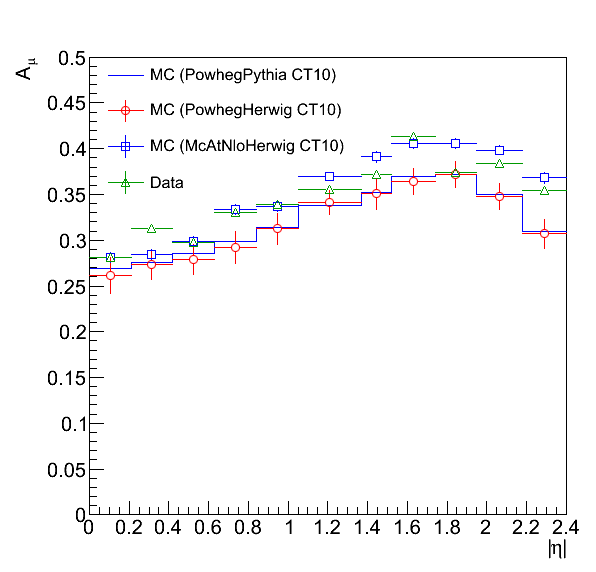
\includegraphics[width=0.65\textwidth]{dates/20130306/figures/asym/Wmn_NORASYM_2D_PT20_POS_Unf_2d_Slice_1}

}

\slide{ $25 < p_T < 30$ }
{

\centering
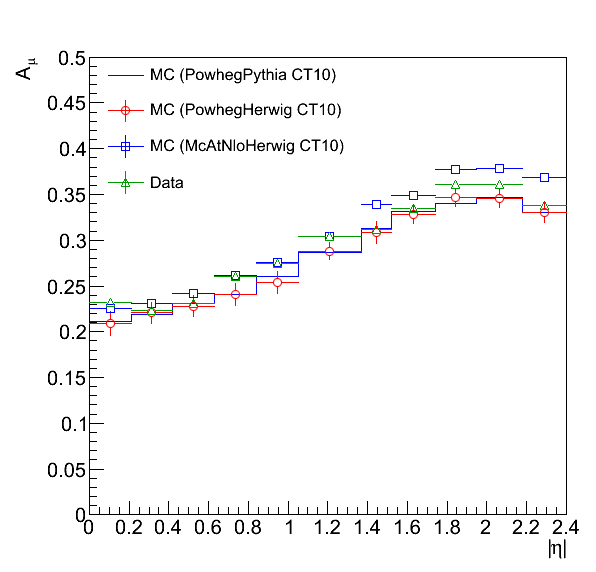
\includegraphics[width=0.65\textwidth]{dates/20130306/figures/asym/Wmn_NORASYM_2D_PT20_POS_Unf_2d_Slice_2}

}

\slide{ $30 < p_T < 35$ }
{

\centering
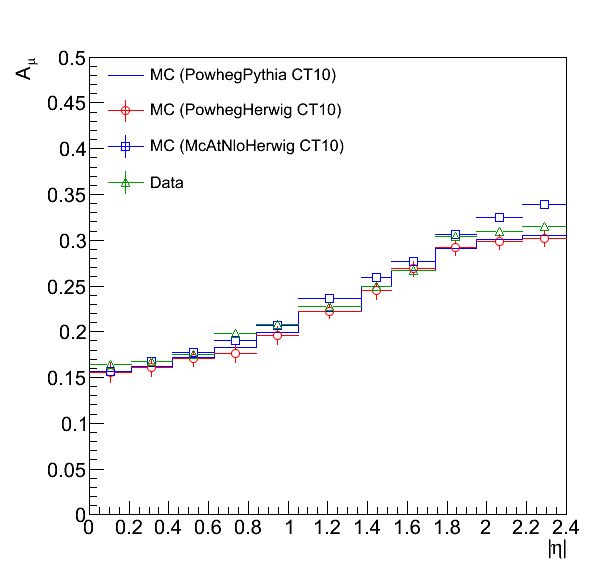
\includegraphics[width=0.65\textwidth]{dates/20130306/figures/asym/Wmn_NORASYM_2D_PT20_POS_Unf_2d_Slice_3}

}

\slide{ $35 < p_T < 40$ }
{

\centering
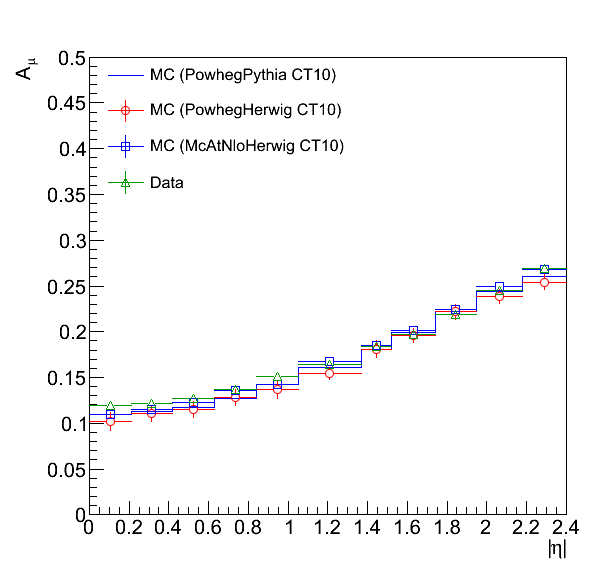
\includegraphics[width=0.65\textwidth]{dates/20130306/figures/asym/Wmn_NORASYM_2D_PT20_POS_Unf_2d_Slice_4}

}

\slide{ $40 < p_T < 45$ }
{

\centering
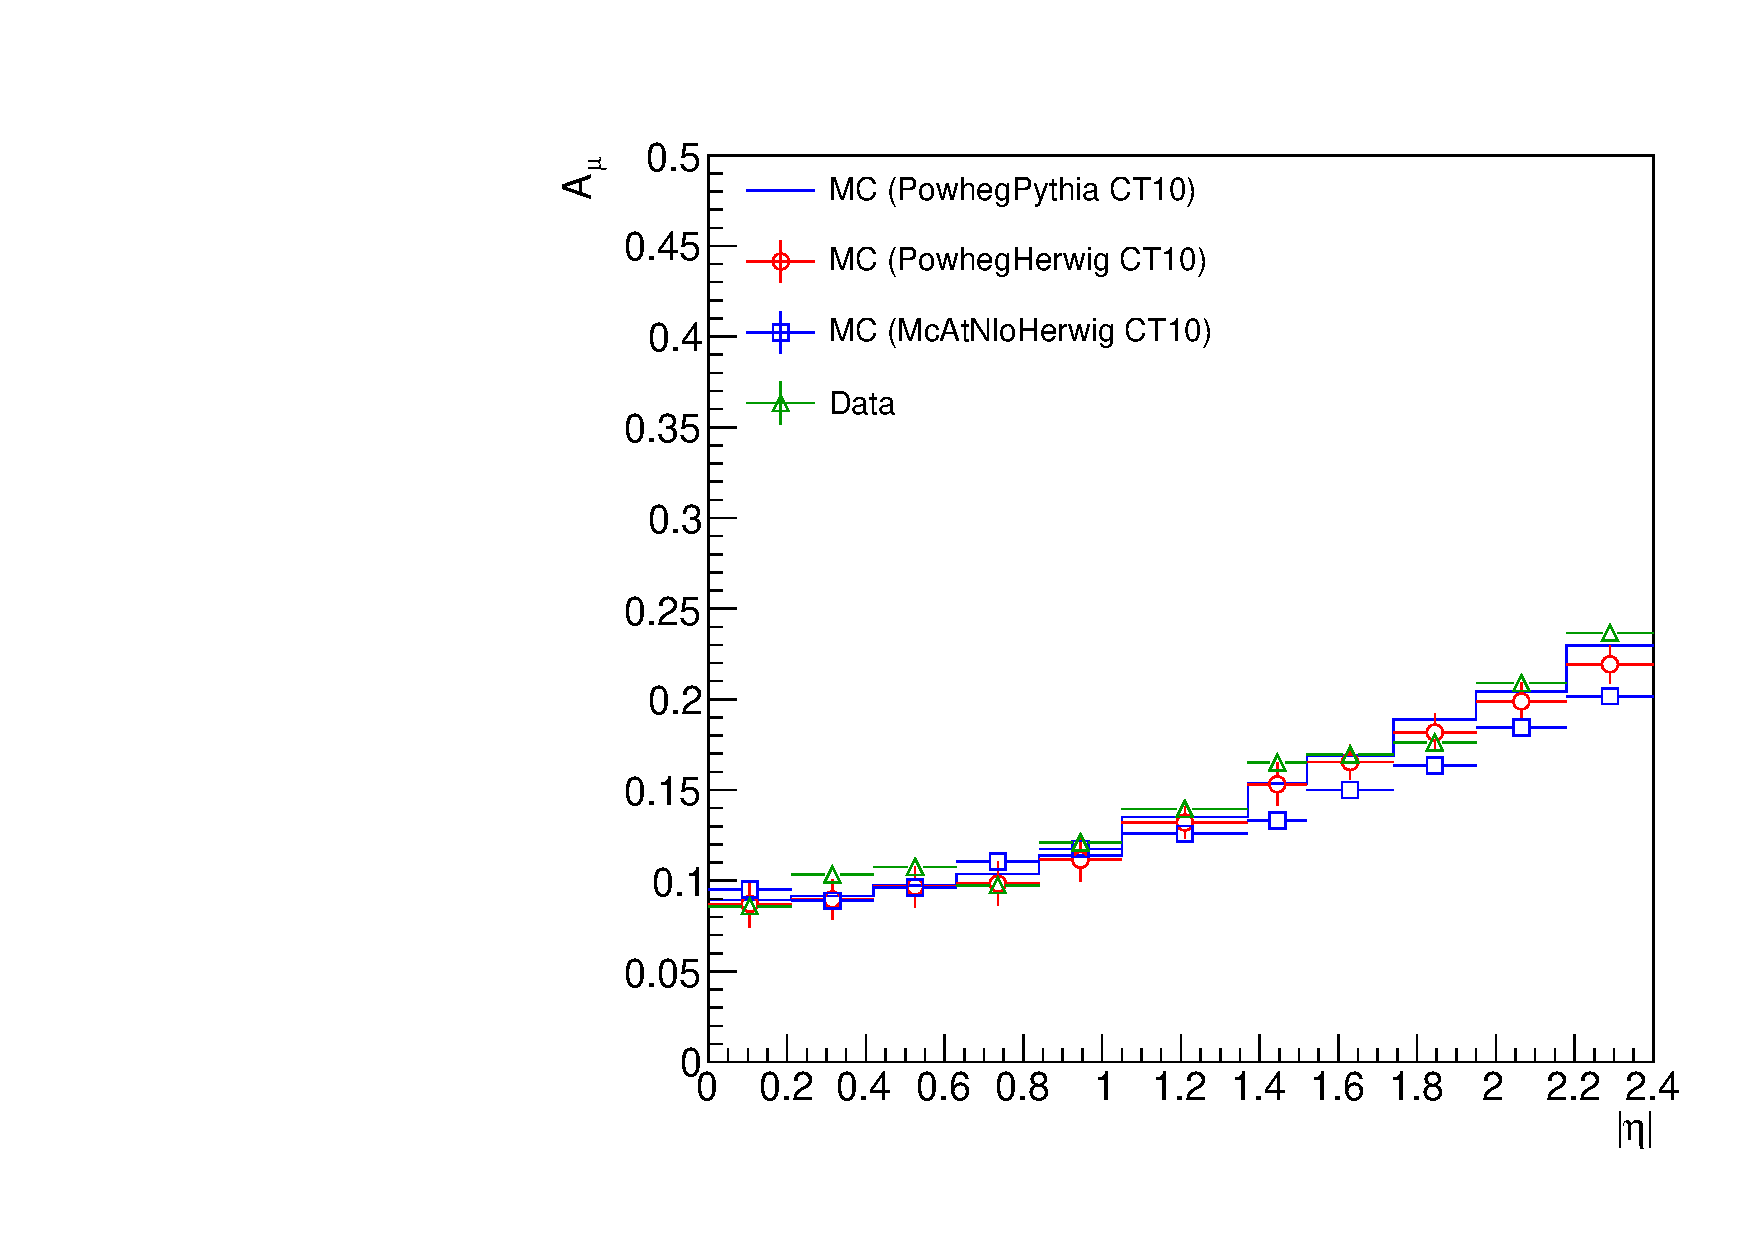
\includegraphics[width=0.65\textwidth]{dates/20130306/figures/asym/Wmn_NORASYM_2D_PT20_POS_Unf_2d_Slice_5}

}

\slide{ $45 < p_T < 50$ }
{

\centering
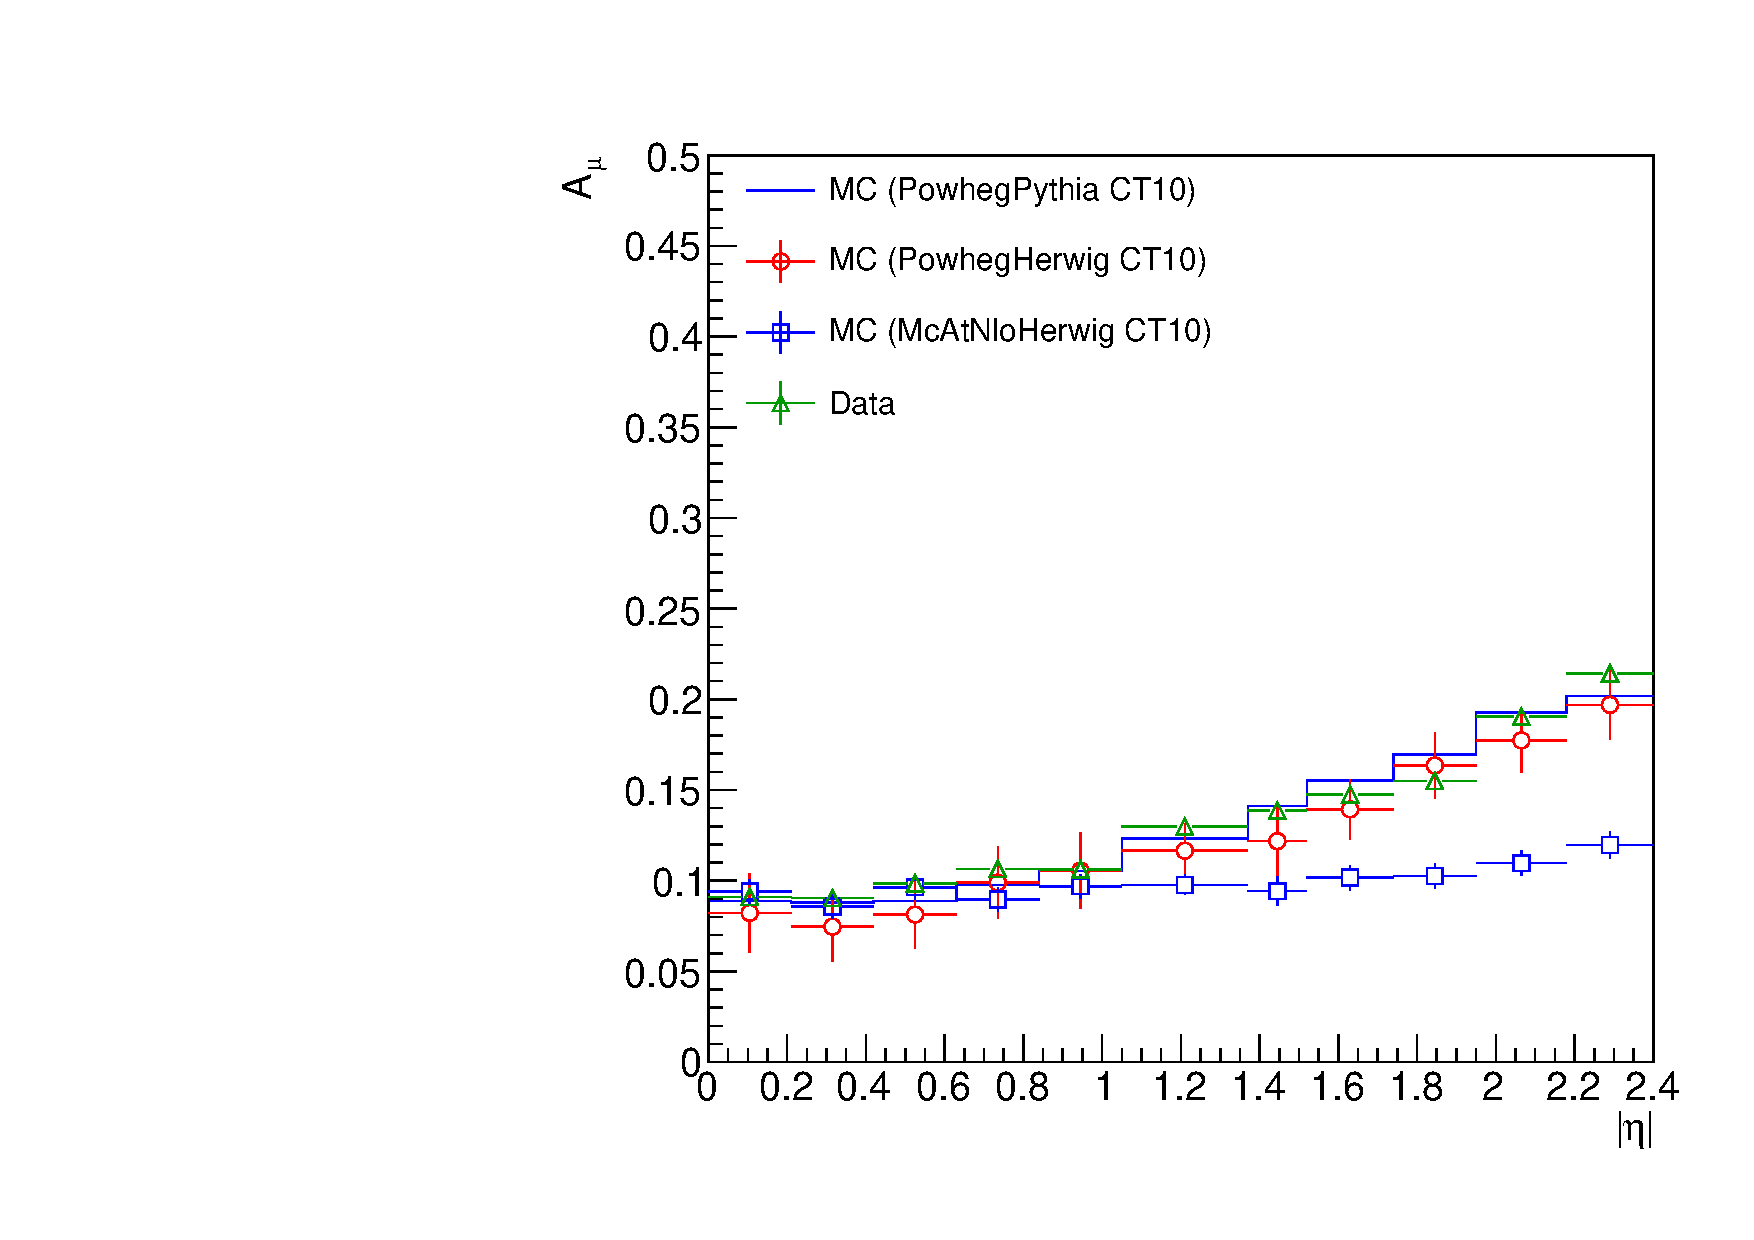
\includegraphics[width=0.65\textwidth]{dates/20130306/figures/asym/Wmn_NORASYM_2D_PT20_POS_Unf_2d_Slice_6}

}

\slide{ $p_T > 50$ }
{

\centering
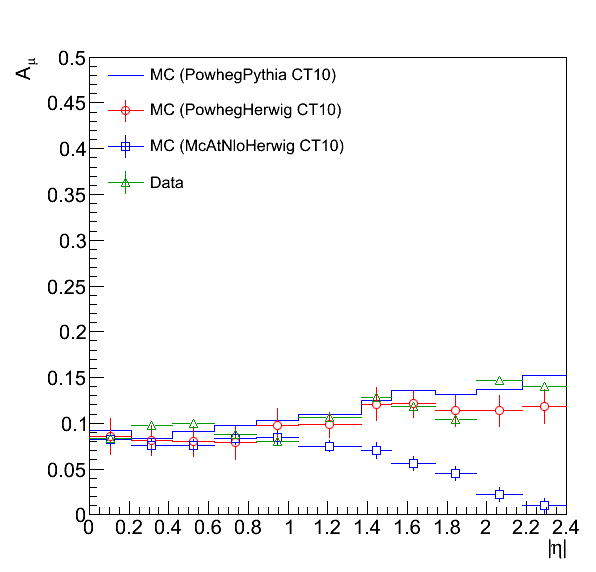
\includegraphics[width=0.65\textwidth]{dates/20130306/figures/asym/Wmn_NORASYM_2D_PT20_POS_Unf_2d_Slice_7}

}


%%%%%%% Back-up slides %%%%%%%%%%
\appendix
\newcounter{finalframe}
\setcounter{finalframe}{\value{framenumber}}

\slide{}
{

\centering
\Huge Back-up slides
}
